The next section describes a project made in collaboration with
Jessica Ody, 
Guillaume Buisson-Chavot, 
Anthony Cnudde.
Code and an detailed description can be found on \url{https://github.com/ancnudde/Artificial_intelligence}.

As described by \cite{loos2019},
periplasmic proteins can be distinguished from cytoplasmic ones based on other features than the presence of a signal peptide up to an accuray of at least 95 percent.
The analysis described above confirms that there seem to be many features that distinguish these two protein groups.
Therefore, in our project, we tried to make a predictor that could distinguish periplasmic proteins from cytoplasmic ones.
The dataset including all the Gammaproteobacteria described above was used for this purpose.

Three sets of UniRep vectors were generated:
one for the cytoplasmic protein sequences,
one for the periplasmic protein sequences including the signal peptide,
and one for the periplasmic protein sequences excluding the signal peptide. 
Fig. \ref{fig:pca_sp} shows a PCA of the cytoplasmic UniRep vectors and periplasmic (including signal peptide) UniRep vectors.
In UniRep feature space,
there is a clear separation between the two groups.
When comparing cytoplasmic UniRep vectores to periplasmic (excluding signal peptide) UniRep vectors (Fig. \ref{fig:pca_without_sp}),
the separation is less clear.

The UniRep vector used for this analysis contained only 64 elements to express biophysical protein features.
The mLSTM RNN did not have additional information except for the protein sequences.
In other words, even though it known that signal peptides indicate the final location of a protein,
for the mLSTM RNN this was just another sequence.
Yet, it still "decided" it was significant to include this information to such a degree in the UniRep vector that a PCA could easily separate periplasmic from cytoplasmic protein sequences when the signal peptide was included.

~\begin{figure}[h!]
	~\begin{subfigure}[b]{0.49\linewidth}
		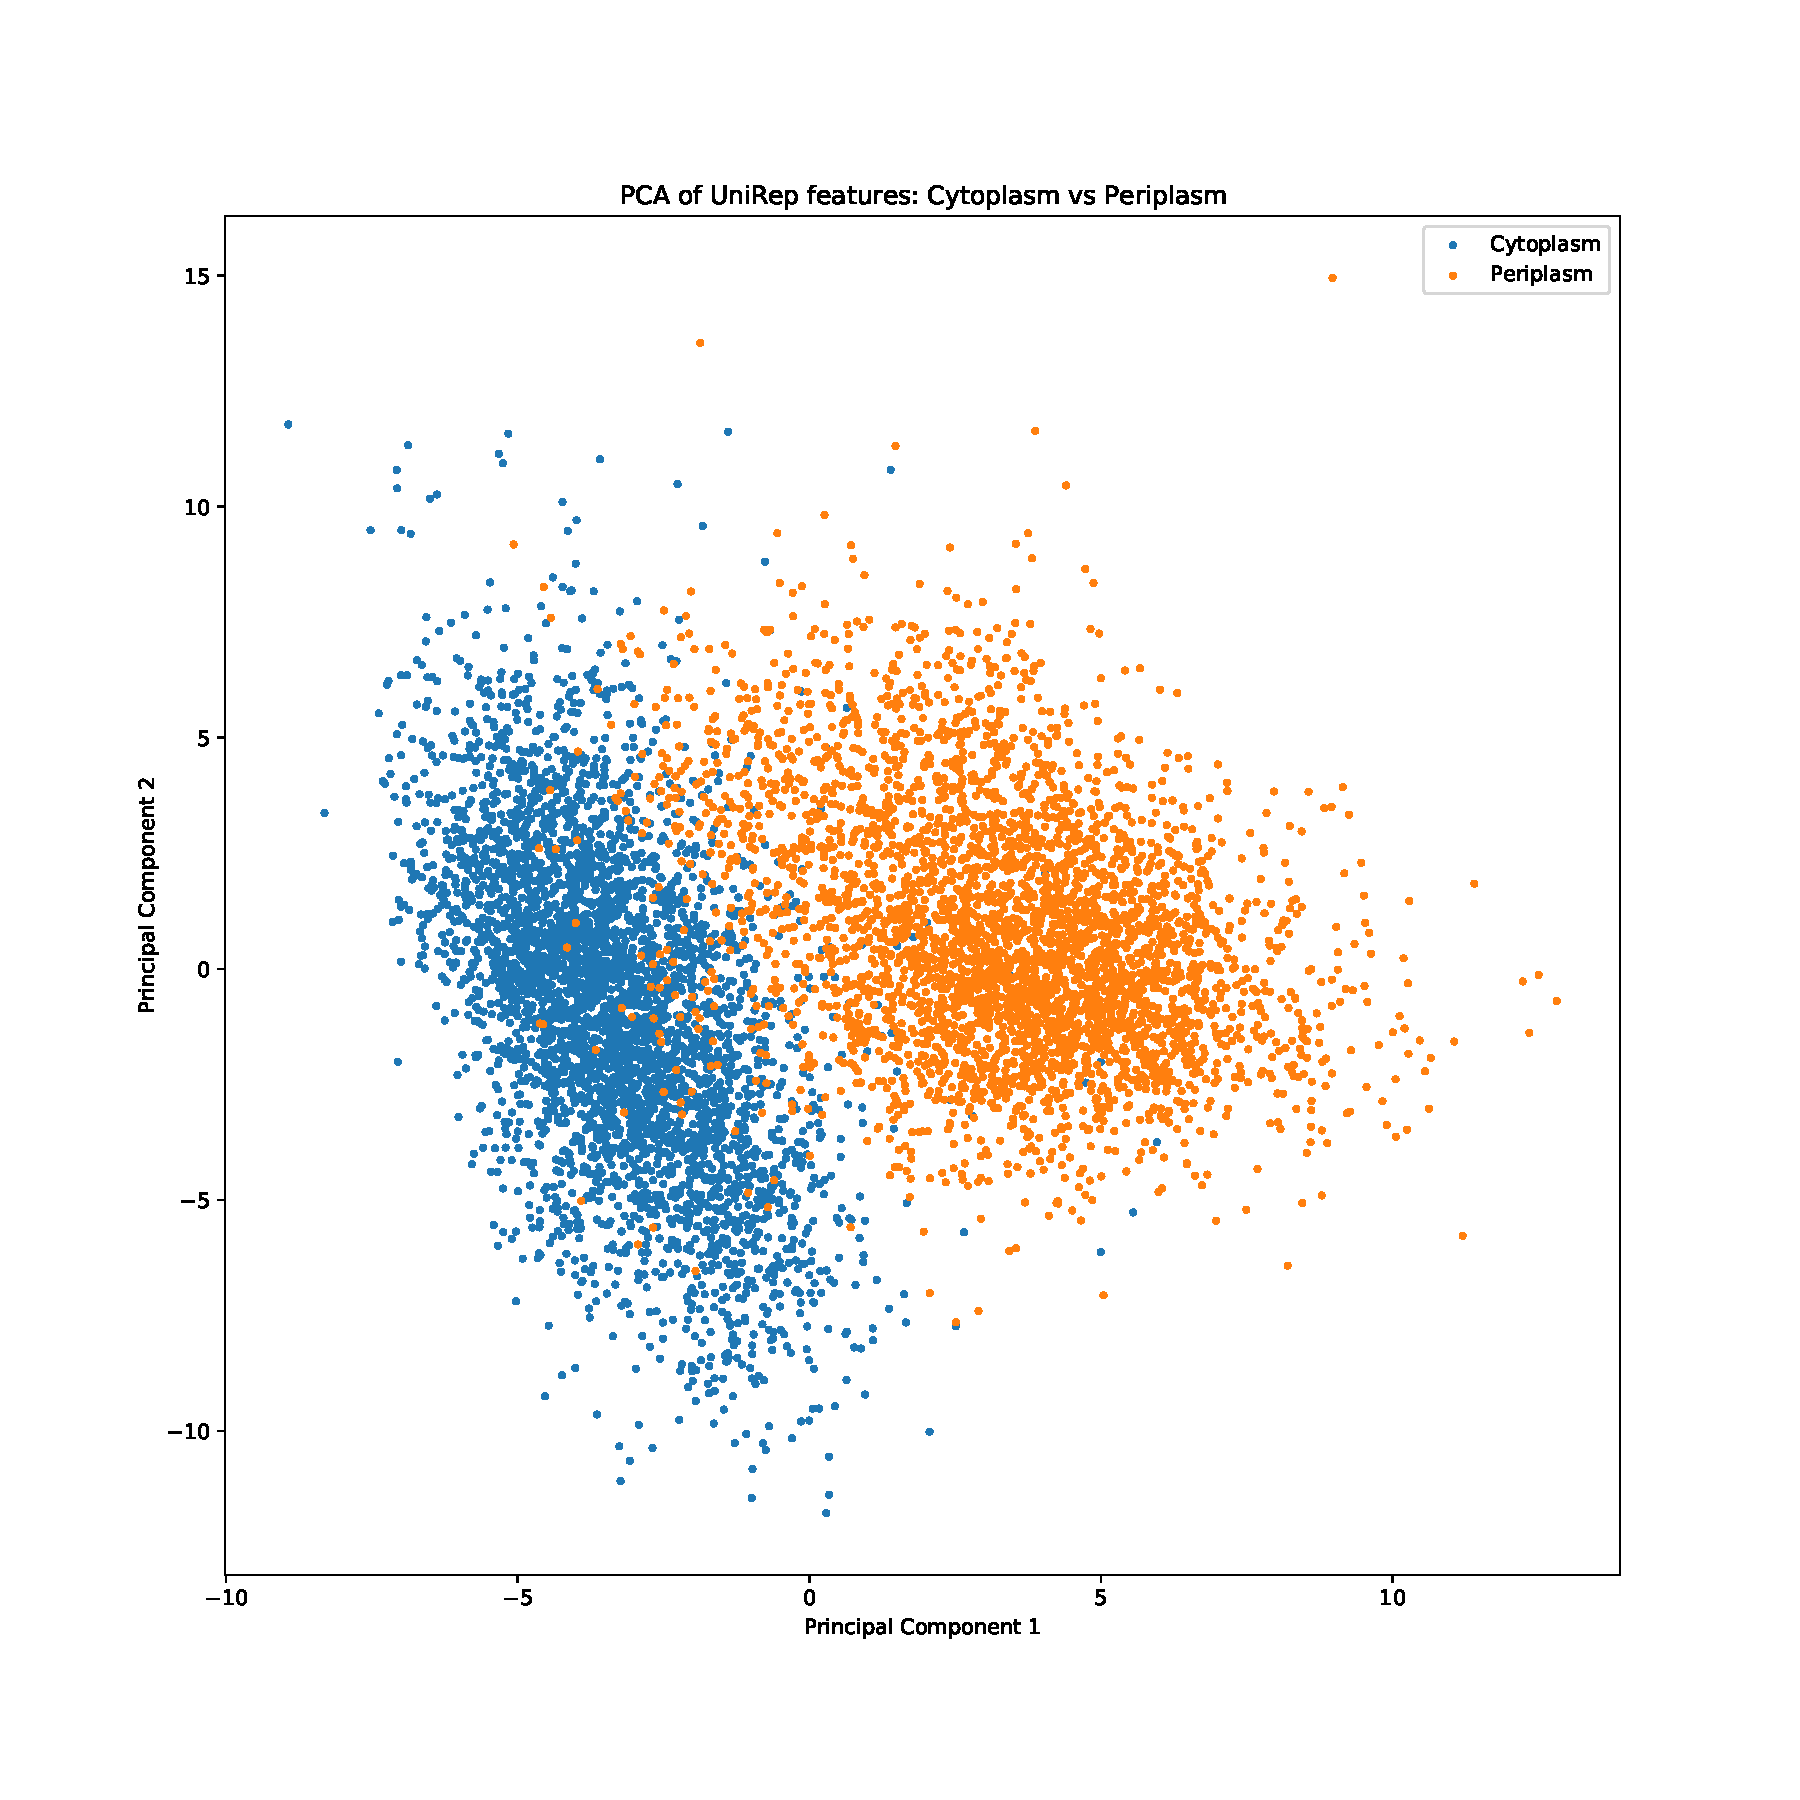
\includegraphics[width=\linewidth]{./results/UniRep/img/pca.pdf}
		\caption{Signal peptide included.}
		\label{fig:pca_sp}
	~\end{subfigure}
	~\begin{subfigure}[b]{0.49\linewidth}
		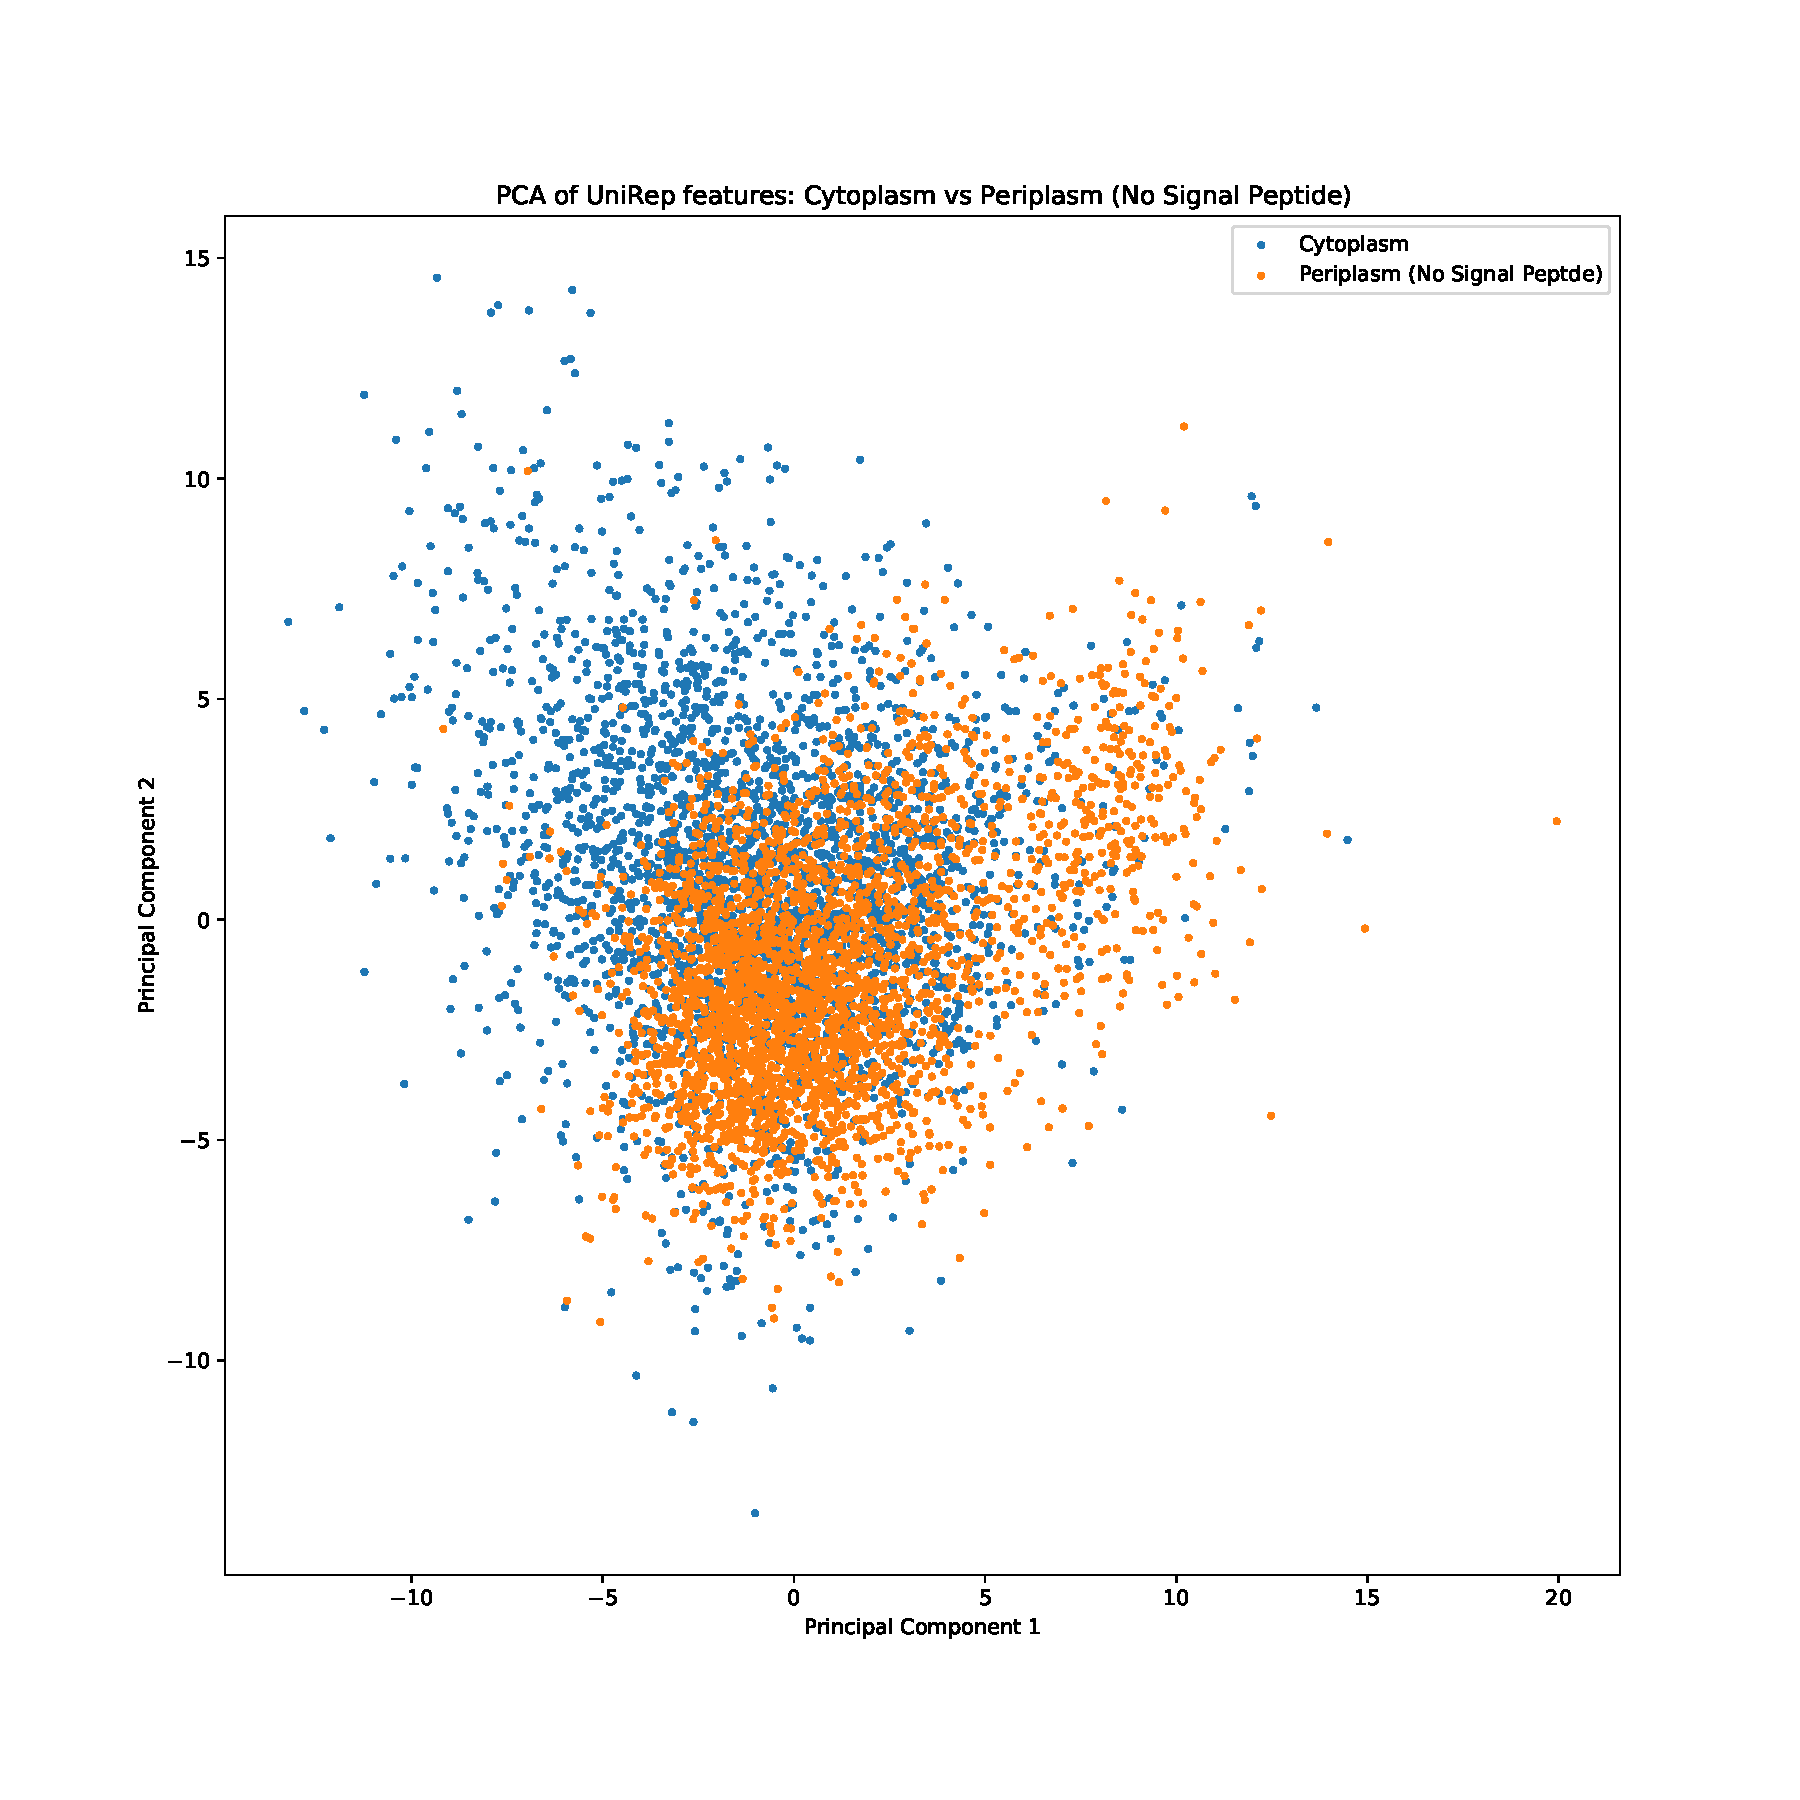
\includegraphics[width=\linewidth]{./results/UniRep/img/pca_without_sp.pdf}
		\caption{Signal peptide excluded.}
		\label{fig:pca_without_sp}
	~\end{subfigure}
	\caption{\textbf{PCA of UniRep space.}}
	\label{fig:pca}
~\end{figure}

Two linear regression based predictors were trained,
one with the inclusion of signal peptides and one without.
The linear regression based predictor that included signal peptides correctly classified 98.7 percent of the test set.
The linear regression based predictor that excluded signal peptides correctly classified 94.8 percent of the test set.
This supports the observation that features in the mature domain are able to distinguish between cytoplasmic and periplasmic protein to a high degree.
In addition to the linear regression based predictor,
a decision tree,
random forest,
support vector machine,
and neural network were trained on the dataset that included the signal peptides (Table. \ref{table:prediction}). 
The neural network gave the best accuracy (99.3 percent).


~\begin{longtable}[]{@{}lll@{}}
\toprule
& include signal peptide & exclude signal peptide\tabularnewline
\midrule
\endhead
Linear regression & 0.987 & 0.948\tabularnewline
Decision tree & 0.981 & \tabularnewline
Radnom forest & 0.977 & \tabularnewline
Neural network & 0.993 &\tabularnewline
SVM & 0.983 & \tabularnewline
\bottomrule
\caption{\textbf{Classification of periplasmic and cytoplasmic protein sequences.}
Accuracy is shown for different ML-methods.}
\label{table:prediction}
~\end{longtable}

It should be noted that this project was part of the \textit{Techniques of artificial intelligence} course.
Therefore the main aim was to create our own implementation of the machine learning methods described above.
Retraining the data on more optimised implementation, for example from the \textit{sklearn} python library could possibly improve the results.
